% Úvod
%%%%%%%%%%%%%%%%%%%%%%%%%%%%%%%%%%%%%%%%%%%%%%%%%%%%%%%%%%%%%%%%%%%%%%%%%%%%%%%%%%%%%%%%%%%%%%
\section{Introduction}
The application MemSkel (\textbf{Mem}brane \textbf{Skel}etonization) is a tool for segmentation of a cell membrane. The process is interactive which means that a user guidance is necessary. The user has to mark (with the mouse) at least one point in the image. These marked points are called seeds. After the segmentation is done it is possible to edit obtained result manually with Eraser tool. When the user is satisfied with the segmentation the skeletonization can be run. This process finds the medial axis of the segmentation mask. For this to work, the segmentation mask must be closed otherwise the skeletonization will fail. The output of the skeletonization (the skelet) can be further approximated using b-spline with variable smoothing parameter.

\begin{figure}[htb]
    \centering
    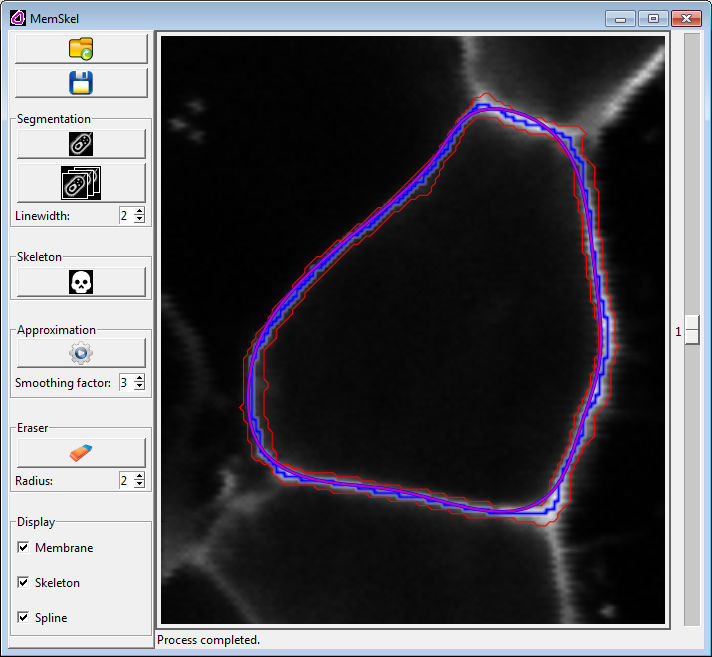
\includegraphics[width = .7\linewidth]{gui.png}
    \caption{The main window of the application.}
    \label{fig:gui}
\end{figure}

% Graphical User Interface
%%%%%%%%%%%%%%%%%%%%%%%%%%%%%%%%%%%%%%%%%%%%%%%%%%%%%%%%%%%%%%%%%%%%%%%%%%%%%%%%%%%%%%%%%%%%%%
\section{Graphical User Interface} \label{sec:stEd}
The application consists of the main parts: tool window, visualisation. In this section individual components of the GUI are described. The components are numbered as follows:
 \ref{fig:gui_labeled}.

\begin{figure}[htb]
    \centering
    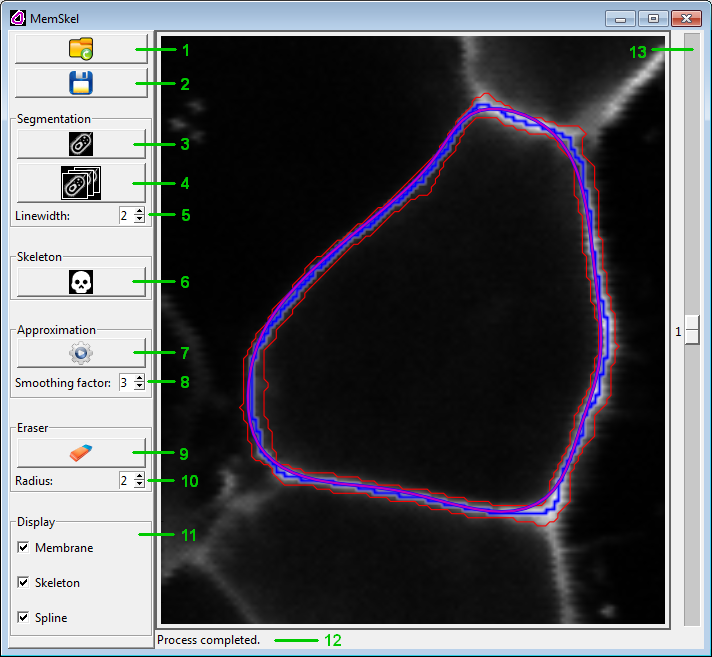
\includegraphics[width = .7\textwidth]{gui_labeled.png}
    \caption{The main window with numbered components.}
    \label{fig:gui_labeled}
\end{figure}

The numbered main components from figure \ref{fig:gui_labeled} are described bellow:
\begin{enumerate}
    \item Open file \ldots opens a dialogue window for loading data from a file.
	\item Save \ldots opens a dialogue window for saving the results.
	\item Segmentation of a frame \ldots segments actual frame.
	\item Segmentation of the stack \ldots segments all frames (pages) in data.
	\item Linewidth \ldots spinbox for changing the width of line, which is used for marking the membrane.
	\item Skeletonization \ldots runs the skeletonization procedure to get the medial axis of the membrane mask.
	\item Approximation \ldots runs the approximation of the medial axis with the smoothing parameter given by the spinbox bellow.
	\item Smoothing factor \ldots spinbox for changing the smoothing factor that is used in approximation.
	\item Eraser \ldots runs process for deleting points from the membrane mask.
	\item Radius \ldots spinbox for changing the Eraser radius.
	\item Display \ldots checkboxes for enabling/disabling visualisation of appropriate parts.
	\item Status bar \ldots displays information about the state of the application.
	\item Slider \ldots allows the user to change data frame.
\end{enumerate}


% Use of the application
%%%%%%%%%%%%%%%%%%%%%%%%%%%%%%%%%%%%%%%%%%%%%%%%%%%%%%%%%%%%%%%%%%%%%%%%%%%%%%%%%%%%%%%%%%%%%%
\section{Use of the Application}
This section refers to individual components with numbers that corresponds to the figure \ref{fig:gui_labeled} and the list above. The references are hold in circles with the number inside it, e.g. the reference of the button for opening a file has the form \circled{1}.

%%%%%%%%%%%%%%%%%%%%%%%%%%%%%%%%%%%%%%%%%%%%%%%%%%%%%%%%%%%%%%%%%%%%%%%%%%%%%%%%%%%%%%%%%%%%%%
\subsection{Running and Closing}
To start the application the file \textit{memSkel\_main.exe } needs to be runned. Traditionally, the application terminates by clicking the red cross button in upper right corner of the main window.

%%%%%%%%%%%%%%%%%%%%%%%%%%%%%%%%%%%%%%%%%%%%%%%%%%%%%%%%%%%%%%%%%%%%%%%%%%%%%%%%%%%%%%%%%%%%%%
\subsection{Loading the Data}
By clicking the button \circled{1} the file dialogue for opening a file pops up. At this moment, only TIFF format for the input data is supported. The data format should be complete, i.e. it should contain metainformation about frame size. If you're not able to open data, re-saving it another image viewer/editor  should help. This way the missing data should be filled in. One such an editor is \textit{IrfanView}. Another approach that could help is to save the data in 8-bit format.

When the data is loaded, they are shown in the editor.

%%%%%%%%%%%%%%%%%%%%%%%%%%%%%%%%%%%%%%%%%%%%%%%%%%%%%%%%%%%%%%%%%%%%%%%%%%%%%%%%%%%%%%%%%%%%%%
\subsection{Segmentation of Cell Membrane}
As already mentioned, the segmentation procedure needs to know at least one point (seed) that belongs to the membrane. The mode for marking the seed points is ran by clicking the button \circled{3} or \circled{4}. After that the user can mark points by moving the mouse when the left mouse button is held down. After hitting the Enter key, the algorithm starts segmenting the rest of the membrane. After the algorithm terminates the user is able to supply more seeds and rerun the segmentation process (again by the Enter key).

To end the segmentation process, you must wait until the algorithm terminates. After that just press Enter without providing any other seed points. Then it is possible to use the Eraser to delete areas outside the membrane.

During the editation mode it is possible to change the line width with the spinbox \circled{5} or by the mouse wheel. This way you can provide the algorithm with more points or achieve higher precision by thinning the line.

Clicking the button \circled{4} segments the whole stack, i.e. all frames or pages. In this case, segmentation of the first frame is the same as described above. After segmenting the actual frame, the segmentation starts to grow to other frames. To do this, the algorithm needs to know the skeleton, therefore its computation is ran automatically. The editing of the segmented mask is possible after all frames are segmented.

%%%%%%%%%%%%%%%%%%%%%%%%%%%%%%%%%%%%%%%%%%%%%%%%%%%%%%%%%%%%%%%%%%%%%%%%%%%%%%%%%%%%%%%%%%%%%%
\subsection{Eraser Tool}
Using the Eraser tool it is possible to edit the binary mask of the membrane. If you press the key \circled{9} then a blue circle around the mouse cursor will appear. The size of the circle represents area that is affected by the Eraser and could be changed by the spinbox \circled{10} or by the mouse wheel. By holding the left mouse button the erasing mode starts, which is indicated by change of the circle color from blue to red, see figure \ref{fig:eraser}. When erasing, all pixels of the membrane that are located inside the circle will be erased from the mask, i.e. marked as pixels that do not belong to the membrane. The user can hold down the left mouse button and move it to perform "erasing on the move".

\begin{figure}[htb]
	\centering
	\subfloat[]{\label{fig:eraserA}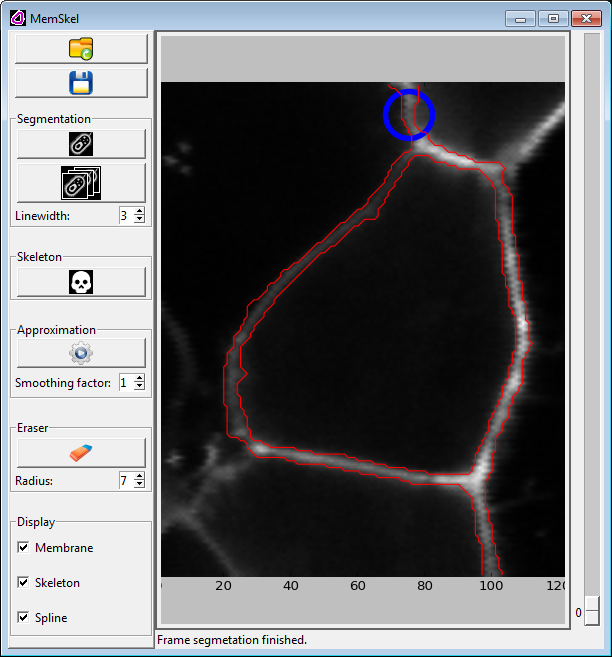
\includegraphics[width=0.45\textwidth]{eraser3.png}}
	\hskip 0.1cm
	\subfloat[]{\label{fig:eraserB}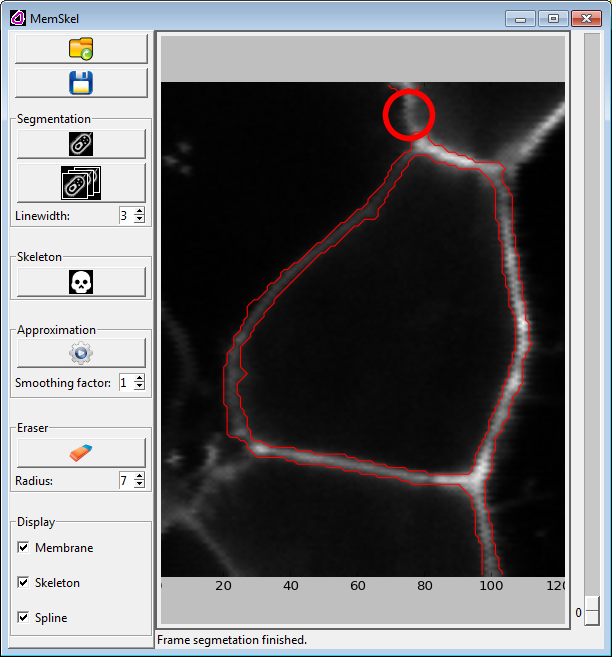
\includegraphics[width=0.45\textwidth]{eraser4.png}}
	\caption{The use of the Eraser tool. The figure. \ref{fig:eraserA} shows the erasing mode, figure \ref{fig:eraserB} shows situation when the user holds down the left mouse button.}
	\label{fig:eraser}
\end{figure}

%%%%%%%%%%%%%%%%%%%%%%%%%%%%%%%%%%%%%%%%%%%%%%%%%%%%%%%%%%%%%%%%%%%%%%%%%%%%%%%%%%%%%%%%%%%%%%
\subsection{Skeletonization}
The next step after the membrane is found is to define its medial axis, i.e. its skeleton. This process is triggered by hitting the button \circled{6}. The membrane needs to be closed otherwise the skeletonization yields a one-point skeleton, see fig. \ref{fig:skel}.

\begin{figure}[htb]
	\centering
	\subfloat[]{\label{fig:skelA1}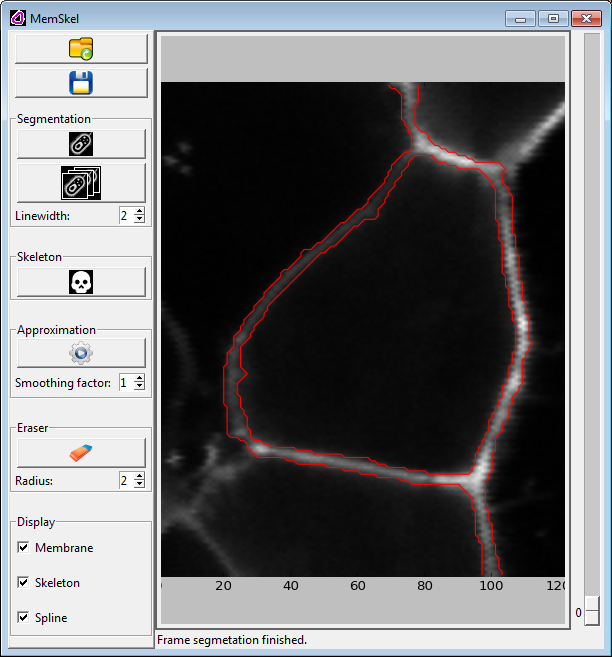
\includegraphics[width=0.45\textwidth]{skelA1.png}}
	\hskip 0.1cm
	\subfloat[]{\label{fig:skelA2}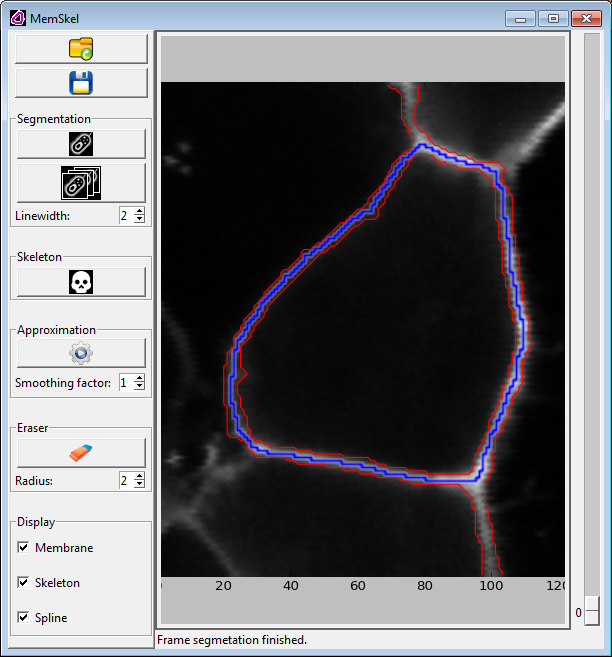
\includegraphics[width=0.45\textwidth]{skelA2.png}}
	\\
	\subfloat[]{\label{fig:skelB1}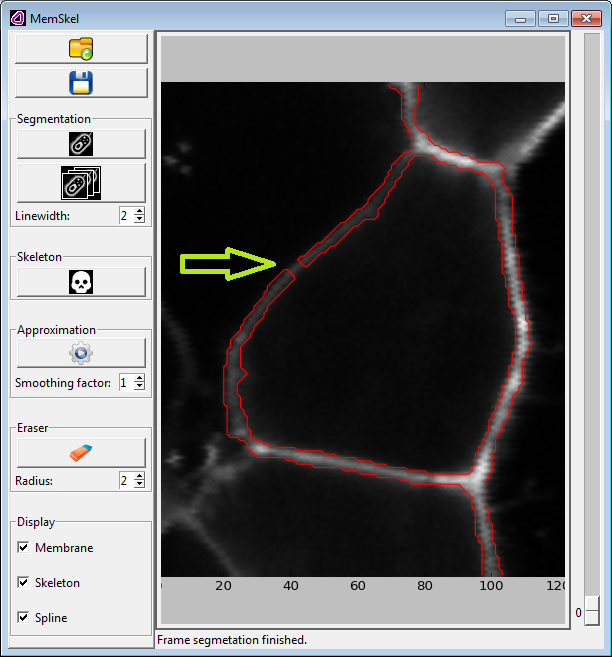
\includegraphics[width=0.45\textwidth]{skelB1.png}}
	\hskip 0.1cm
	\subfloat[]{\label{fig:skelB2}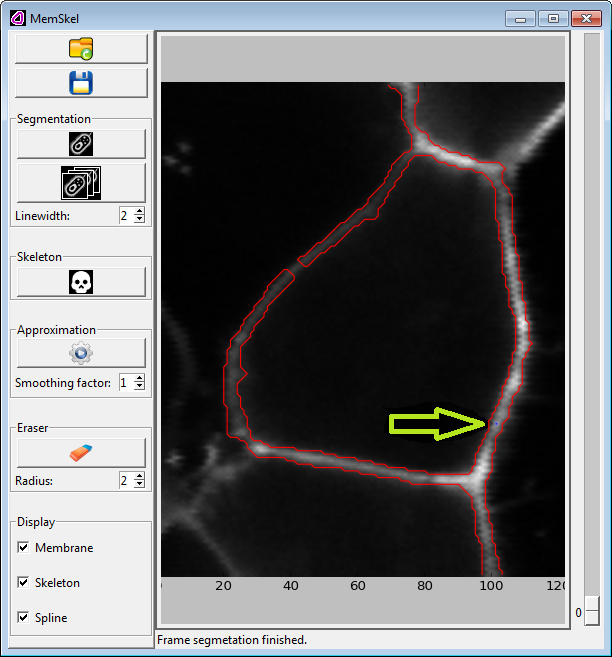
\includegraphics[width=0.45\textwidth]{skelB2.png}}
	\caption{An example of the skeletonization. Fig. \ref{fig:skelA1} shows right segmented membrane and its skeleton is shown in \ref{fig:skelA2}. If the membrane is not closed, see fig. \ref{fig:skelB1}, the skeleton will end like an point as shown in fig. \ref{fig:skelB2}.}
	\label{fig:skel}
\end{figure}

%%%%%%%%%%%%%%%%%%%%%%%%%%%%%%%%%%%%%%%%%%%%%%%%%%%%%%%%%%%%%%%%%%%%%%%%%%%%%%%%%%%%%%%%%%%%%%
\subsection{Approximation}
The skeleton can be further approximated by a b-spline by clicking on the button \circled{7}. The user is also able to define the smoothness factor by the spinbox \circled{8}. An example showing the use of approximation is shown in fig. \ref{fig:spline}.

\begin{figure}[htb]
	\centering
	\subfloat[]{\label{fig:spline1}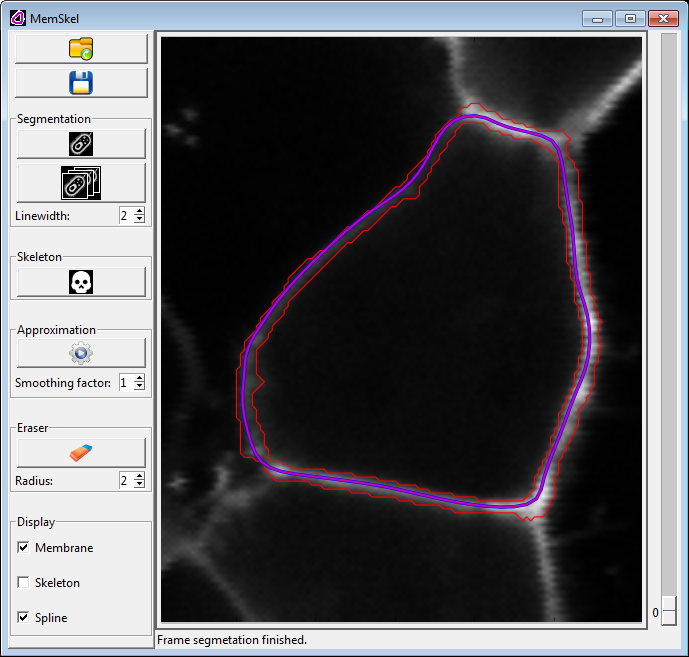
\includegraphics[width=0.45\textwidth]{app1.png}}
	\hskip 0.1cm
	\subfloat[]{\label{fig:spline2}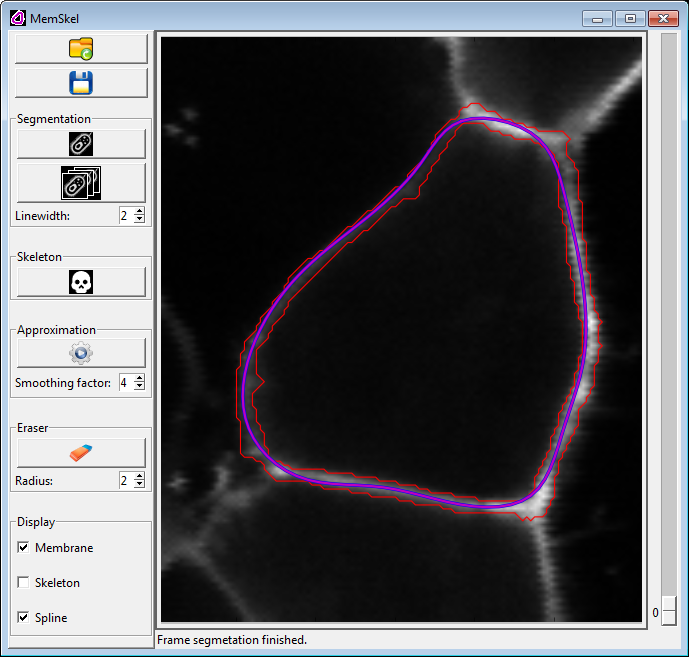
\includegraphics[width=0.45\textwidth]{app4.png}}
	\\
	\subfloat[]{\label{fig:spline3}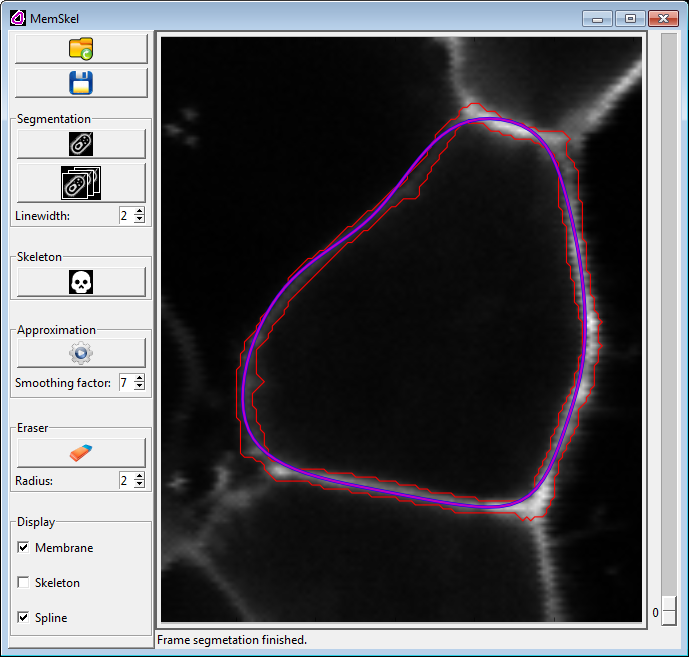
\includegraphics[width=0.45\textwidth]{app7.png}}
	\hskip 0.1cm
	\subfloat[]{\label{fig:spline4}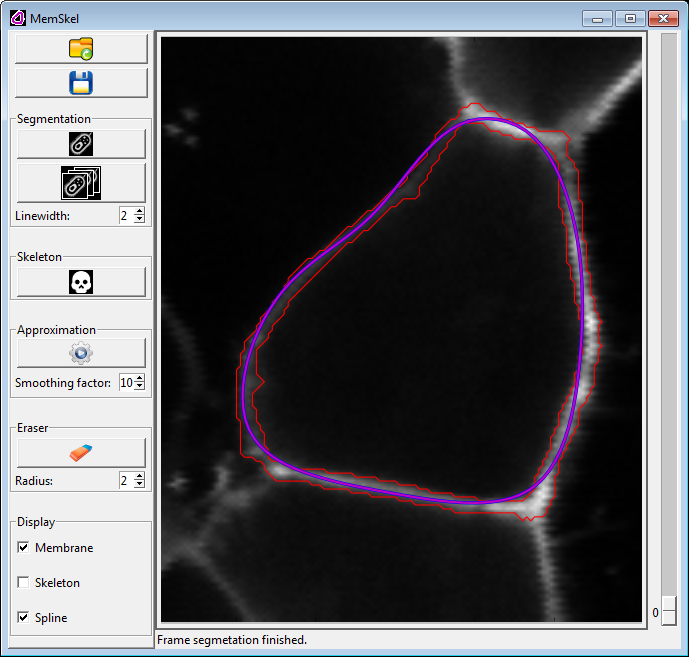
\includegraphics[width=0.45\textwidth]{app10.png}}
	\caption{An example of the approximation of the skeleton with different smoothing factor: factor = 1 ... \ref{fig:spline1}, factor = 4 ... \ref{fig:spline2}, factor = 7 ... \ref{fig:spline3} a factor = 10 ... \ref{fig:spline4}.}
	\label{fig:spline}
\end{figure}

%%%%%%%%%%%%%%%%%%%%%%%%%%%%%%%%%%%%%%%%%%%%%%%%%%%%%%%%%%%%%%%%%%%%%%%%%%%%%%%%%%%%%%%%%%%%%%
\subsection{Saving the results}
To save the results the user needs to click the button \circled{2}. After that the software creates two files:
\begin{enumerate}
	\item binary image defining the segmented membrane, 
	\item text file describing the parameters of the approximating spline.
\end{enumerate}

% Ostatní
%%%%%%%%%%%%%%%%%%%%%%%%%%%%%%%%%%%%%%%%%%%%%%%%%%%%%%%%%%%%%%%%%%%%%%%%%%%%%%%%%%%%%%%%%%%%%%
\section{Miscellaneous}

\subsection{Status bar}
The status bar \circled{12} shows main information about running processes in the editor, e.g. information about successful/unsuccessful data loading and saving, process flow etc. When segmenting multiframe data, the right part of the status bar shows a progress bar. It informs the user what part of data was already processed and what part remains. 

\subsection{Log file}
If the software ends with a critical error, a window pops up that informs the user about logging the error in log file. This file is named \textit{memskel\_main.exe.log} and provide more information about the error. This file is extremely important for the developers to debug the software.

%\subsection{Podporované OS}
%Editor je vytvořen na operačním systému Windows, současné podporované verze jsou Win 7 a Win XP. Editor funguje jak na 32-bitových tak i na 64-bitových operačních systémech.
% Ostatní
%%%%%%%%%%%%%%%%%%%%%%%%%%%%%%%%%%%%%%%%%%%%%%%%%%%%%%%%%%%%%%%%%%%%%%%%%%%%%%%%%%%%%%%%%%%%%%
\section{Running the software from source}
This section describes how to install and run the software.
\subsection{Required packages}
The software uses several packages that are listed here. Used package version is also provided.
\begin{itemize}
	\item Python 2.7.5
	\item numpy-MKL-1.7.1
	\item scipy-0.12.0
	\item matplotlib-1.1.1 (newer version doesn't work), before installation you need to install following packages:
		\begin{itemize}
			\item python-dateutil-1.5
			\item pytz-2013b
			\item pyparsing-1.5.7
		\end{itemize}
	\item pylibtiff-0.3.0.dev82
	\item Pillov-2.0.0
\end{itemize}

%------------------------------------------------------------------------------
\subsection{Order of installing packages}
An order of installing the packages needs to be fulfilled, otherwise the software might not work.
\begin{enumerate}
	\item python-2.7.5.msi \ldots installs the Python itself; it does not matter if you install 32 or 64 bit version as long as you installed the same bit version of all following packages,
	\item numpy-MKL-1.7.1.win32-py2.7.exe \ldots working with n-dimensional arrays,
	\item scipy-0.12.0.win32-py2.7.exe \ldots for approximation of the skeleton,
	\item python-dateutil-1.5.win32-py2.7.exe \ldots prerequisite of the matplotlib package,
	\item pytz-2013b.win32-py2.7.exe \ldots prerequisite of the matplotlib package,
	\item pyparsing-1.5.7.win32-py2.7.exe \ldots prerequisite of the matplotlib package,
	\item matplotlib-1.1.1.win32-py2.7.exe \ldots visualization, more recent version might not work,
	\item pylibtiff-0.3.0.dev82.win32-py2.7.exe \ldots working with TIFF images,
	\item Pillow-2.0.0.win32-py2.7.exe \ldots image processing,
	\item setuptools-0.7.4.win32-py2.7.exe \ldots instalation of packages from source codes,
	\item pymorph-0.96 \ldots morphological operations; installation is described bellow.
\end{enumerate}

For installation of the \textit{pymorph} package it is necessary to add the Python do system variable PATH. Some package may to do that automatically during its installation - in that case this step is not necessary. To verify if the Python is in the system PATH you can do the following:
\begin{enumerate}
	\item run command line, e.g. with \textit{Win+R} and writing \textit{cmd} as in fig. \ref{fig:run_cmd},
	\item write \textit{python --help} in the command line - some text about python command should be displayed as in fig \ref{fig:cmd_python_help_OK}.
	\item if some text is shown as in fig. \ref{fig:cmd_python_help_OK}, the Python is in your system PATH,
	\item if a text sayng that Python is unknown command is shown (\ref{fig:cmd_python_help_KO}), Python is not in you system Path and you need to put it there, e.g. with command \textit{setx path "\%path\%;c:$\backslash$Python27"}; information about successful operation should be shown (\ref{fig:cmd_python_added}); after restarting the command line an repeating the step 2 should provide you with successful message.
\end{enumerate}

\begin{figure}[htb]
	\centering
	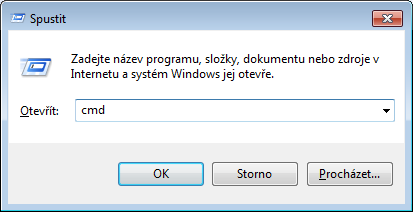
\includegraphics[width=0.4\textwidth]{spustit_cmd.png}
	\caption{Running the command line.}
	\label{fig:run_cmd}
\end{figure}

\begin{figure}[htb]
	\centering
	\subfloat[Python is in system PATH]{\label{fig:cmd_python_help_OK}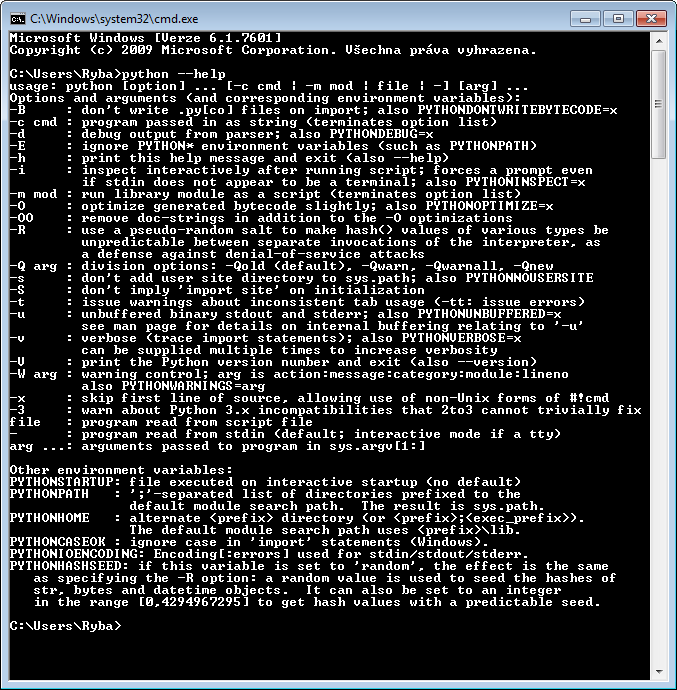
\includegraphics[width=0.45\textwidth]{cmd_python_help_OK.png}}
	\hskip 0.2cm
	\subfloat[Python is not in system PATH]{\label{fig:cmd_python_help_KO}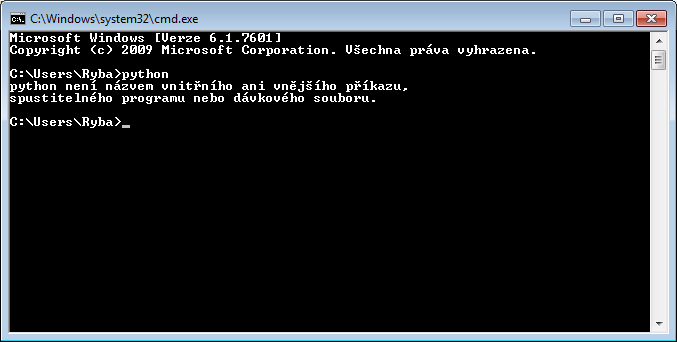
\includegraphics[width=0.45\textwidth]{cmd_python_help_KO.png}}
	\caption{Checking whether the Python is in your system PATH variable.}
	\label{fig:cmd_python_help}
\end{figure}

\begin{figure}[htb]
	\centering
	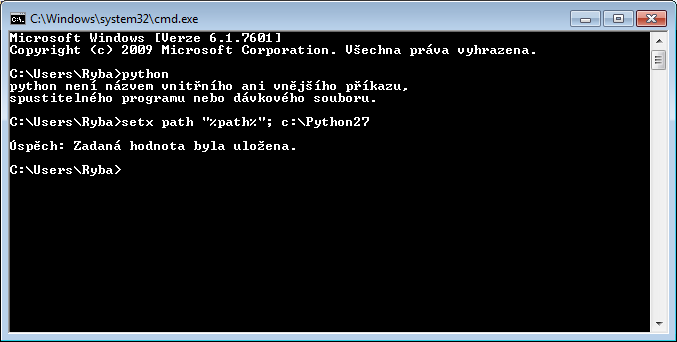
\includegraphics[width=0.4\textwidth]{cmd_python_added.png}
	\caption{Adding Python to the system PATH.}
	\label{fig:cmd_python_added}
\end{figure}

When the Python is in the system PATH you can install the package \textit{pymorhp} with the \textit{setuptools}. It is necessary in command line to get inside a directory \textit{pymorph-0.96}. Then you can run the installation with the command \textit{python setup.py install}. When the installation is successful, the command line should inform you with a successful message(\ref{fig:cmd_pymorph}).

\begin{figure}[htb]
	\centering
	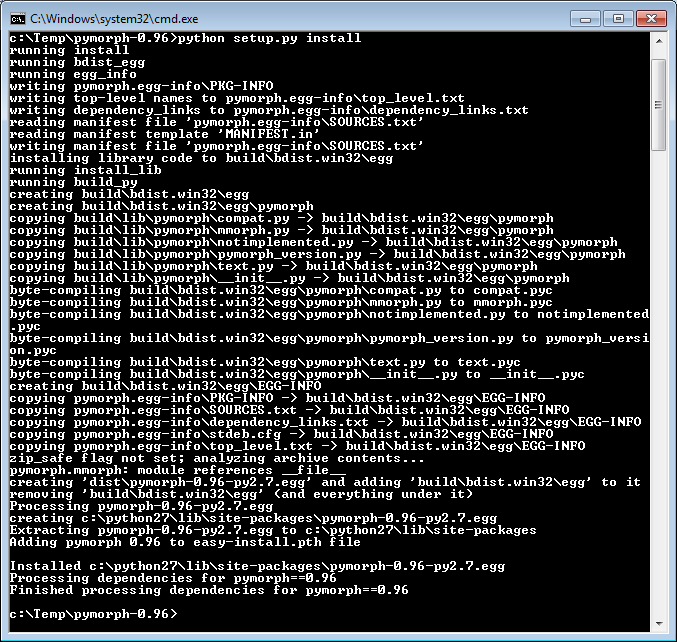
\includegraphics[width=0.4\textwidth]{cmd_pymorph.png}
	\caption{Instalation of the package \textit{pymorph}.}
	\label{fig:cmd_pymorph}
\end{figure}

%------------------------------------------------------------------------------
\subsection{Running the software}
If the Python is in the system PATH (it should be), it is possible to run the MemSkel with file \textit{memSkel\_main.py}. Eventually it is possible to run it from the command line with command  \textit{python memSkel\_main.py}, but you need to be inside the directory which contains the file \textit{memSkel\_main.py}, see fig. \ref{fig:run}.

\begin{figure}[htb]
	\centering
	
\includegraphics[width=0.4\textwidth]{run.png}
	\caption{Running the software MemSkel from the command line.}
	\label{fig:run}
\end{figure}